\newpage
\null
\thispagestyle{empty}
\newpage
\addcontentsline{toc}{chapter}{Mark}
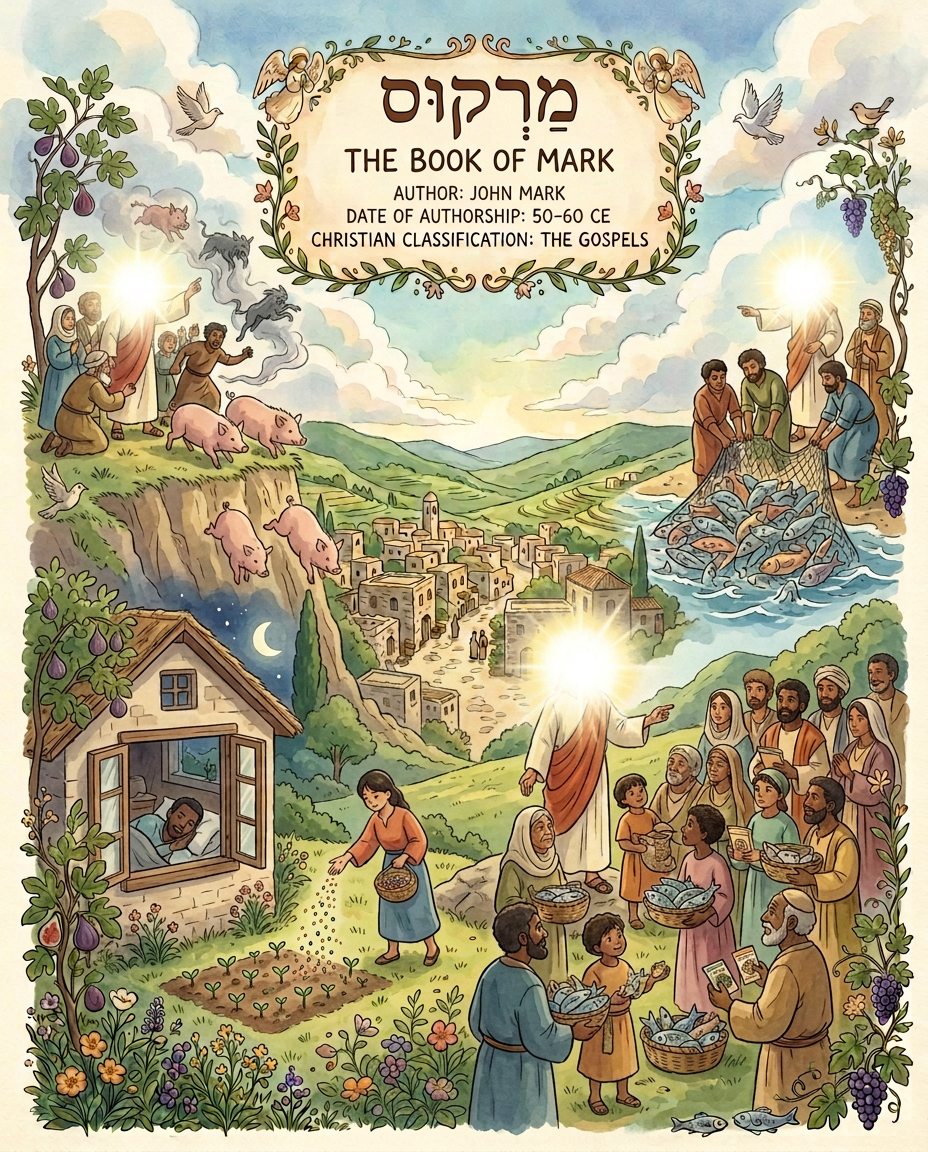
\includepdf[pages=1, fitpaper=false, width=\paperwidth, height=\paperheight, , keepaspectratio=false]{images/divider2/mark2.png}
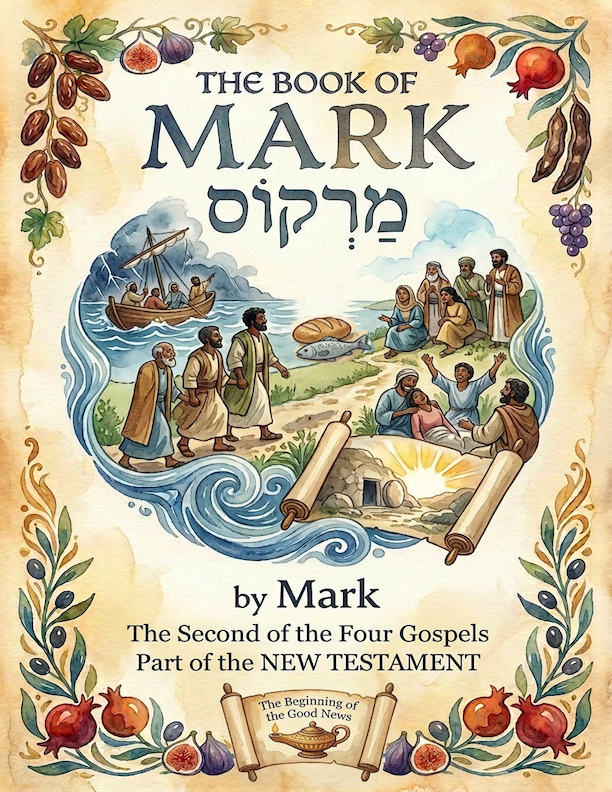
\includepdf[pages=1, fitpaper=false, width=\paperwidth, height=\paperheight, , keepaspectratio=false]{images/divider1/mark.png}

\includepdf[pages=1, fitpaper=false, width=\paperwidth, height=\paperheight, , keepaspectratio=false]{images/8.5x11-Dot-Grid.png}

\includepdf[pages=1, fitpaper=false, width=\paperwidth, height=\paperheight, , keepaspectratio=false]{images/8.5x11-Dot-Grid.png}

\mybook{Mark}
\vspace{-1.36in}

\mychapter{} \myverse*{}The beginning of the Good News of Yeshua the Messiah, the Son of
God.

\myverse{}As it is written in the Prophets,

“Behold,\footnote{1:2 “Behold”, from “ἰδοὺ”, means look at, take notice, observe, see, or gaze at. It is often used
	as an interjection.} I send my messenger before your face,

who will prepare your way before you:\footnote{1:2 Malachi 3:1}

\myverse{}the voice of one crying in the wilderness,

‘Make ready the way of the Lord!

Make his paths straight!’ ”\footnote{1:3 Isaiah 40:3}

\myverse{}Yochanan came immersing\footnote{1:4 or, immersing} in the wilderness and proclaiming the immersion of repentance for forgiveness
of sins.
\myverse{}All the country of Judea and all those of Jerusalem went out to him. They were
immersed by him in the Jordan river, confessing their sins.
\myverse{}Yochanan was clothed with camel’s hair and a leather belt around his waist.
He ate locusts and wild honey.
\myverse{}He preached, saying, “After me comes he who is mightier than I, the strap of
whose sandals I am not worthy to stoop down and loosen.
\myverse{}I immersed you in\footnote{1:8 The Greek word (en) translated here as “in” could also be translated as “with” in some contexts.}
water, but he will immerse you in the Holy Spirit.”

\myverse{}In those days, Yeshua came from Nazareth of Galilee, and was immersed
by Yochanan in the Jordan.
\myverse{}Immediately coming up from the water, he saw the heavens parting and the Spirit
descending on him like a dove.
\myverse{}A voice came out of the sky, “You are my beloved Son, in whom I am well pleased.”

\myverse{}Immediately the Spirit drove him out into the wilderness.
\myverse{}He was there in the wilderness forty days, tempted by Satan. He was with the
wild animals; and the angels were serving him.

\myverse{}Now after Yochanan was taken into custody, Yeshua came into Galilee,
proclaiming the Good News of God’s Kingdom,
\myverse{}and saying,
\textcolor{crimson}{“The time is fulfilled, and God’s Kingdom is at hand! Repent, and believe in the Good News.”}

\myverse{}Passing along by the sea of Galilee, he saw Simon and Andrew,
the brother of Simon, casting a net into the sea, for they were fishermen.
\myverse{}Yeshua said to them,
\textcolor{crimson}{“Come after me, and I will make you into fishers for men.”}

\myverse{}Immediately they left their nets, and followed him.

\myverse{}Going on a little further from there, he saw Jacob the son of
Zebedee, and Yochanan his brother, who were also in the boat mending the nets.
\myverse{}Immediately he called them, and they left their father, Zebedee, in the boat
with the hired servants, and went after him.

\myverse{}They went into Capernaum, and immediately on the Sabbath day
he entered into the synagogue and taught.
\myverse{}They were astonished at his teaching, for he taught them as having authority,
and not as the scribes.
\myverse{}Immediately there was in their synagogue a man with an unclean spirit, and
he cried out,
\myverse{}saying, “Ha! What do we have to do with you, Yeshua, you Nazarene? Have you
come to destroy us? I know who you are: the Holy One of God!”

\myverse{}Yeshua rebuked him, saying,
\textcolor{crimson}{“Be quiet, and come out of him!”
}

\myverse{}The unclean spirit, convulsing him and crying with a loud voice,
came out of him.
\myverse{}They were all amazed, so that they questioned among themselves, saying, “What
is this? What can this new doctrine be? For with authority he commands even the unclean spirits, and they
obey him!”
\myverse{}The report of him went out immediately into all the region of Galilee and
its surrounding area.

\myverse{}Immediately, when they had come out of the synagogue, they came
into the house of Simon and Andrew, with Jacob and Yochanan.
\myverse{}Now Simon’s wife’s mother lay sick with a fever, and immediately they told
him about her.
\myverse{}He came and took her by the hand and raised her up. The fever left her immediately,\footnote{1:31 NU omits “immediately”.} and she served them.

\myverse{}At evening, when the sun had set, they brought to him all who
were sick and those who were possessed by demons.
\myverse{}All the city was gathered together at the door.
\myverse{}He healed many who were sick with various diseases and cast out many demons.
He didn’t allow the demons to speak, because they knew him.

\myverse{}Early in the morning, while it was still dark, he rose up and
went out, and departed into a deserted place, and prayed there.
\myverse{}Simon and those who were with him searched for him.
\myverse{}They found him and told him, “Everyone is looking for you.”

\myverse{}He said to them,
\textcolor{crimson}{“Let’s go elsewhere into the next towns, that I may proclaim there also, because I came out for this
	reason.”}
\myverse{}He went into their synagogues throughout all Galilee, proclaiming and casting
out demons.

\myverse{}A leper came to him, begging him, kneeling down to him, and saying
to him, “If you want to, you can make me clean.”

\myverse{}Being moved with compassion, he stretched out his hand, and touched
him, and said to him,
\textcolor{crimson}{“I want to. Be made clean.”}
\myverse{}When he had said this, immediately the leprosy departed from him and he was
made clean.
\myverse{}He strictly warned him and immediately sent him out,
\myverse{}and said to him,
\textcolor{crimson}{“See that you say nothing to anybody, but go show yourself to the priest and offer for your cleansing
	the things which Moses commanded, for a testimony to them.”}

\myverse{}But he went out, and began to proclaim it much, and to spread
about the matter, so that Yeshua could no more openly enter into a city, but was outside in desert places.
People came to him from everywhere.


% MARK 2
\mychapter{} \myverse*{}When he entered again into Capernaum after some days, it was heard
that he was at home.
\myverse{}Immediately many were gathered together, so that there was no more room, not
even around the door; and he spoke the word to them.
\myverse{}Four people came, carrying a paralytic to him.
\myverse{}When they could not come near to him for the crowd, they removed the roof where
he was. When they had broken it up, they let down the mat that the paralytic was lying on.
\myverse{}Yeshua, seeing their faith, said to the paralytic,
\textcolor{crimson}{“Son, your sins are forgiven you.”}

\myverse{}But there were some of the scribes sitting there and reasoning
in their hearts,
\myverse{}“Why does this man speak blasphemies like that? Who can forgive sins but God
alone?”

\myverse{}Immediately Yeshua, perceiving in his spirit that they so reasoned
within themselves, said to them,
\textcolor{crimson}{“Why do you reason these things in your hearts?
}
\myverse{}\textcolor{crimson}{Which is easier, to tell the paralytic, ‘Your sins are forgiven;’ or to
	say, ‘Arise, and take up your bed, and walk’?
}
\myverse{}\textcolor{crimson}{But that you may know that the Son of Man has authority on earth to forgive
	sins”}—he said to the paralytic—
\myverse{}\textcolor{crimson}{“I tell you, arise, take up your mat, and go to your house.”
}

\myverse{}He arose, and immediately took up the mat and went out in front
of them all, so that they were all amazed and glorified God, saying, “We never saw anything like this!”

\myverse{}He went out again by the seaside. All the multitude came to him,
and he taught them.
\myverse{}As he passed by, he saw Levi the son of Halfai sitting at the tax office.
He said to him,
\textcolor{crimson}{“Follow me.”} And he arose and followed him.

\myverse{}He was reclining at the table in his house, and many tax collectors
and sinners sat down with Yeshua and his disciples, for there were many, and they followed him.
\myverse{}The scribes and the Pharisees, when they saw that he was eating with the sinners
and tax collectors, said to his disciples, “Why is it that he eats and drinks with tax collectors and
sinners?”

\myverse{}When Yeshua heard it, he said to them,
\textcolor{crimson}{“Those who are healthy have no need for a physician, but those who are sick. I came not to call the
	righteous, but sinners to repentance.”}

\myverse{}Yochanan’s disciples and the Pharisees were fasting, and they
came and asked him, “Why do Yochanan’s disciples and the disciples of the Pharisees fast, but your disciples
don’t fast?”

\myverse{}Yeshua said to them,
\textcolor{crimson}{“Can the groomsmen fast while the bridegroom is with them? As long as they have the bridegroom with
	them, they can’t fast.
}
\myverse{}\textcolor{crimson}{But the days will come when the bridegroom will be taken away from them,
	and then they will fast in that day.
}
\myverse{}\textcolor{crimson}{No one sews a piece of unshrunk cloth on an old garment, or else the patch
	shrinks and the new tears away from the old, and a worse hole is made.
}
\myverse{}\textcolor{crimson}{No one puts new wine into old wineskins; or else the new wine will burst
	the skins, and the wine pours out, and the skins will be destroyed; but they put new wine into fresh wineskins.”}

\myverse{}He was going on the Sabbath day through the grain fields; and
his disciples began, as they went, to pluck the ears of grain.
\myverse{}The Pharisees said to him, “Behold, why do they do that which is not lawful
on the Sabbath day?”

\myverse{}He said to them,
\textcolor{crimson}{“Did you never read what David did when he had need and was hungry—he, and those who were with him?
}
\myverse{}\textcolor{crimson}{How he entered into God’s house at the time of Abiathar the high priest,
	and ate the show bread, which is not lawful to eat except for the priests, and gave also to those who
	were with him?”}

\myverse{}He said to them,
\textcolor{crimson}{“The Sabbath was made for man, not man for the Sabbath.
}
\myverse{}\textcolor{crimson}{Therefore the Son of Man is lord even of the Sabbath.”}


%Mark 3
\mychapter{} \myverse*{}He entered again into the synagogue, and there was a man there
whose hand was withered.
\myverse{}They watched him, whether he would heal him on the Sabbath day, that they might
accuse him.
\myverse{}He said to the man whose hand was withered,
\textcolor{crimson}{“Stand up.”}
\myverse{}He said to them,
\textcolor{crimson}{“Is it lawful on the Sabbath day to do good or to do harm? To save a life or to kill?”} But they
were silent.
\myverse{}When he had looked around at them with anger, being grieved at the hardening
of their hearts, he said to the man,
\textcolor{crimson}{“Stretch out your hand.”
} He stretched it out, and his hand was restored as healthy as the other.
\myverse{}The Pharisees went out, and immediately conspired with the Herodians against
him, how they might destroy him.

\myverse{}Yeshua withdrew to the sea with his disciples; and a great multitude
followed him from Galilee, from Judea,
\myverse{}from Jerusalem, from Idumaea, beyond the Jordan, and those from around Tyre
and Sidon. A great multitude, hearing what great things he did, came to him.
\myverse{}He spoke to his disciples that a little boat should stay near him because of
the crowd, so that they wouldn’t press on him.
\myverse{}For he had healed many, so that as many as had diseases pressed on him that
they might touch him.
\myverse{}The unclean spirits, whenever they saw him, fell down before him and cried,
“You are the Son of God!”
\myverse{}He sternly warned them that they should not make him known.

\myverse{}He went up into the mountain and called to himself those whom
he wanted, and they went to him.
\myverse{}He appointed twelve, that they might be with him, and that he might send them
out to proclaim
\myverse{}and to have authority to heal sicknesses and to cast out demons:
\myverse{}Simon (to whom he gave the name Peter);
\myverse{}Jacob the son of Zebedee; and Yochanan, the brother of Jacob, (whom he called
Benei-Regesh, which means, Sons of Thunder);
\myverse{}Andrew; Philip; Bartholomew; Matthew; Thomas; Jacob, the son of Halfai; Taddai;
Simon the Zealot;
\myverse{}and Judah Iscariot, who also betrayed him.

Then he came into a house.
\myverse{}The multitude came together again, so that they could not so much as eat bread.
\myverse{}When his friends heard it, they went out to seize him; for they said, “He
is insane.”
\myverse{}The scribes who came down from Jerusalem said, “He has Beelzebul,” and, “By
the prince of the demons he casts out the demons.”

\myverse{}He summoned them and said to them in parables,
\textcolor{crimson}{“How can Satan cast out Satan?
}
\myverse{}\textcolor{crimson}{If a kingdom is divided against itself, that kingdom cannot stand.
}
\myverse{}\textcolor{crimson}{If a house is divided against itself, that house cannot stand.
}
\myverse{}\textcolor{crimson}{If Satan has risen up against himself, and is divided, he can’t stand,
	but has an end.
}
\myverse{}\textcolor{crimson}{But no one can enter into the house of the strong man to plunder unless
	he first binds the strong man; then he will plunder his house.
}

\myverse{}\textcolor{crimson}{“Most certainly I tell you, all sins of the descendants of
	man will be forgiven, including their blasphemies with which they may blaspheme;
}
\myverse{}\textcolor{crimson}{but whoever may blaspheme against the Holy Spirit never has forgiveness,
	but is subject to eternal condemnation.”}\footnote{3:29 NU reads, guilty of an eternal sin.}
\myverse{}—because they said, “He has an unclean spirit.”

\myverse{}His mother and his brothers came, and standing outside, they
sent to him, calling him.
\myverse{}A multitude was sitting around him, and they told him, “Behold, your mother,
your brothers, and your sisters\footnote{3:32 TR omits “your sisters”} are outside looking for you.”

\myverse{}He answered them,
\textcolor{crimson}{“Who are my mother and my brothers?”}
\myverse{}Looking around at those who sat around him, he said,
\textcolor{crimson}{“Behold, my mother and my brothers!
}
\myverse{}\textcolor{crimson}{For whoever does the will of God is my brother, my sister, and mother.”}


% MARK 4
\mychapter{} \myverse*{}Again he began to teach by the seaside. A great multitude was gathered
to him, so that he entered into a boat in the sea and sat down. All the multitude were on the land by
the sea.
\myverse{}He taught them many things in parables, and told them in his teaching,
\myverse{}\textcolor{crimson}{“Listen! Behold, the farmer went out to sow.
}
\myverse{}\textcolor{crimson}{As he sowed, some seed fell by the road, and the birds}\footnote{4:4 TR adds “of the air”}
\textcolor{crimson}{came and devoured it.
}
\myverse{}\textcolor{crimson}{Others fell on the rocky ground, where it had little soil, and immediately
	it sprang up, because it had no depth of soil.
}
\myverse{}\textcolor{crimson}{When the sun had risen, it was scorched; and because it had no root, it
	withered away.
}
\myverse{}\textcolor{crimson}{Others fell among the thorns, and the thorns grew up and choked it, and
	it yielded no fruit.
}
\myverse{}\textcolor{crimson}{Others fell into the good ground and yielded fruit, growing up and increasing.
	Some produced thirty times, some sixty times, and some one hundred times as much.”}
\myverse{}He said,
\textcolor{crimson}{“Whoever has ears to hear, let him hear.”}

\myverse{}When he was alone, those who were around him with the twelve
asked him about the parables.
\myverse{}He said to them,
\textcolor{crimson}{“To you is given the mystery of God’s Kingdom, but to those who are outside, all things are done in
	parables,
}
\myverse{}\textcolor{crimson}{that ‘seeing they may see and not perceive, and hearing they may hear
	and not understand, lest perhaps they should turn again, and their sins should be forgiven them.’ ”}\footnote{4:12 Isaiah 6:9-10}

\myverse{}He said to them,
\textcolor{crimson}{“Don’t you understand this parable? How will you understand all of the parables?
}
\myverse{}\textcolor{crimson}{The farmer sows the word.
}
\myverse{}\textcolor{crimson}{The ones by the road are the ones where the word is sown; and when they
	have heard, immediately Satan comes and takes away the word which has been sown in them.
}
\myverse{}\textcolor{crimson}{These in the same way are those who are sown on the rocky places, who,
	when they have heard the word, immediately receive it with joy.
}
\myverse{}\textcolor{crimson}{They have no root in themselves, but are short-lived. When oppression
	or persecution arises because of the word, immediately they stumble.
}
\myverse{}\textcolor{crimson}{Others are those who are sown among the thorns. These are those who have
	heard the word,
}
\myverse{}\textcolor{crimson}{and the cares of this age, and the deceitfulness of riches, and the lusts
	of other things entering in choke the word, and it becomes unfruitful.
}
\myverse{}\textcolor{crimson}{Those which were sown on the good ground are those who hear the word,
	accept it, and bear fruit, some thirty times, some sixty times, and some one hundred times.”}

\myverse{}He said to them,
\textcolor{crimson}{“Is a lamp brought to be put under a basket
}\footnote{4:21 literally, a modion, a dry measuring basket containing about a peck (about 9 liters)}
\textcolor{crimson}{or under a bed? Isn’t it put on a stand?
}
\myverse{}\textcolor{crimson}{For there is nothing hidden except that it should be made known, neither
	was anything made secret but that it should come to light.
}
\myverse{}\textcolor{crimson}{If any man has ears to hear, let him hear.”}

\myverse{}He said to them,
\textcolor{crimson}{“Take heed what you hear. With whatever measure you measure, it will be measured to you; and more
	will be given to you who hear.
}
\myverse{}\textcolor{crimson}{For whoever has, to him more will be given; and he who doesn’t have, even
	that which he has will be taken away from him.”}

\myverse{}He said,
\textcolor{crimson}{“God’s Kingdom is as if a man should cast seed on the earth,
}
\myverse{}\textcolor{crimson}{and should sleep and rise night and day, and the seed should spring up
	and grow, though he doesn’t know how.
}
\myverse{}\textcolor{crimson}{For the earth bears fruit by itself: first the blade, then the ear, then
	the full grain in the ear.
}
\myverse{}\textcolor{crimson}{But when the fruit is ripe, immediately he puts in the sickle, because
	the harvest has come.”}

\myverse{}He said,
\textcolor{crimson}{“How will we liken God’s Kingdom? Or with what parable will we illustrate it?
}
\myverse{}\textcolor{crimson}{It’s like a grain of mustard seed, which, when it is sown in the earth,
	though it is less than all the seeds that are on the earth,
}
\myverse{}\textcolor{crimson}{yet when it is sown, grows up and becomes greater than all the herbs,
	and puts out great branches, so that the birds of the sky can lodge under its shadow.”}

\myverse{}With many such parables he spoke the word to them, as they were
able to hear it.
\myverse{}Without a parable he didn’t speak to them; but privately to his own disciples
he explained everything.

\myverse{}On that day, when evening had come, he said to them,
\textcolor{crimson}{“Let’s go over to the other side.”}
\myverse{}Leaving the multitude, they took him with them, even as he was, in the boat.
Other small boats were also with him.
\myverse{}A big wind storm arose, and the waves beat into the boat, so much that the
boat was already filled.
\myverse{}He himself was in the stern, asleep on the cushion; and they woke him up and
asked him, “Rabbi, don’t you care that we are dying?”

\myverse{}He awoke and rebuked the wind, and said to the sea,
\textcolor{crimson}{“Peace! Be still!”} The wind ceased and there was a great calm.
\myverse{}He said to them,
\textcolor{crimson}{“Why are you so afraid? How is it that you have no faith?”}

\myverse{}They were greatly afraid and said to one another, “Who then is
this, that even the wind and the sea obey him?”


% MARK 5
\mychapter5} \myverse*{}They came to the other side of the sea, into the country of the
Gadarenes.
\myverse{}When he had come out of the boat, immediately a man with an unclean spirit met
him out of the tombs.
\myverse{}He lived in the tombs. Nobody could bind him any more, not even with chains,
\myverse{}because he had been often bound with fetters and chains, and the chains had
been torn apart by him, and the fetters broken in pieces. Nobody had the strength to tame him.
\myverse{}Always, night and day, in the tombs and in the mountains, he was crying out,
and cutting himself with stones.
\myverse{}When he saw Yeshua from afar, he ran and bowed down to him,
\myverse{}and crying out with a loud voice, he said, “What have I to do with you, Yeshua,
you Son of the Most High God? I adjure you by God, don’t torment me.”
\myverse{}For he said to him,
\textcolor{crimson}{“Come out of the man, you unclean spirit!”
}

\myverse{}He asked him,
\textcolor{crimson}{“What is your name?”}

He said to him, “My name is Legion, for we are many.”
\myverse{}He begged him much that he would not send them away out of the country.
\myverse{}Now on the mountainside there was a great herd of pigs feeding.
\myverse{}All the demons begged him, saying, “Send us into the pigs, that we may enter
into them.”

\myverse{}At once Yeshua gave them permission. The unclean spirits came
out and entered into the pigs. The herd of about two thousand rushed down the steep bank into the sea,
and they were drowned in the sea.
\myverse{}Those who fed the pigs fled, and told it in the city and in the country.

The people came to see what it was that had happened.
\myverse{}They came to Yeshua, and saw him who had been possessed by demons sitting,
clothed, and in his right mind, even him who had the legion; and they were afraid.
\myverse{}Those who saw it declared to them what happened to him who was possessed by
demons, and about the pigs.
\myverse{}They began to beg him to depart from their region.

\myverse{}As he was entering into the boat, he who had been possessed by
demons begged him that he might be with him.
\myverse{}He didn’t allow him, but said to him,
\textcolor{crimson}{“Go to your house, to your friends, and tell them what great things the Lord has done for you and
	how he had mercy on you.”}

\myverse{}He went his way, and began to proclaim in Decapolis how Yeshua
had done great things for him, and everyone marveled.

\myverse{}When Yeshua had crossed back over in the boat to the other side,
a great multitude was gathered to him; and he was by the sea.
\myverse{}Behold, one of the rulers of the synagogue, Jairus by name, came; and seeing
him, he fell at his feet
\myverse{}and begged him much, saying, “My little daughter is at the point of death.
Please come and lay your hands on her, that she may be made healthy, and live.”

\myverse{}He went with him, and a great multitude followed him, and they
pressed upon him on all sides.
\myverse{}A certain woman who had a discharge of blood for twelve years,
\myverse{}and had suffered many things by many physicians, and had spent all that she
had, and was no better, but rather grew worse,
\myverse{}having heard the things concerning Yeshua, came up behind him in the crowd
and touched his clothes.
\myverse{}For she said, “If I just touch his clothes, I will be made well.”
\myverse{}Immediately the flow of her blood was dried up, and she felt in her body that
she was healed of her affliction.

\myverse{}Immediately Yeshua, perceiving in himself that the power had
gone out from him, turned around in the crowd and asked,
\textcolor{crimson}{“Who touched my clothes?”}

\myverse{}His disciples said to him, “You see the multitude pressing against
you, and you say, ‘Who touched me?’ ”

\myverse{}He looked around to see her who had done this thing.
\myverse{}But the woman, fearing and trembling, knowing what had been done to her, came
and fell down before him, and told him all the truth.

\myverse{}He said to her,
\textcolor{crimson}{“Daughter, your faith has made you well. Go in peace, and be cured of your disease.”}

\myverse{}While he was still speaking, people came from the synagogue ruler’s
house, saying, “Your daughter is dead. Why bother the Rabbi any more?”

\myverse{}But Yeshua, when he heard the message spoken, immediately said
to the ruler of the synagogue,
\textcolor{crimson}{“Don’t be afraid, only believe.”}
\myverse{}He allowed no one to follow him except Peter, Jacob, and Yochanan the brother
of Jacob.
\myverse{}He came to the synagogue ruler’s house, and he saw an uproar, weeping, and
great wailing.
\myverse{}When he had entered in, he said to them,
\textcolor{crimson}{“Why do you make an uproar and weep? The child is not dead, but is asleep.”}

\myverse{}They ridiculed him. But he, having put them all out, took the
father of the child, her mother, and those who were with him, and went in where the child was lying.
\myverse{}Taking the child by the hand, he said to her,
\textcolor{crimson}{“Talitha cumi!”
} which means, being interpreted,
\textcolor{crimson}{“Girl, I tell you, get up!”
}
\myverse{}Immediately the girl rose up and walked, for she was twelve years old. They
were amazed with great amazement.
\myverse{}He strictly ordered them that no one should know this, and commanded that
something should be given to her to eat.


% MARK 6
\mychapter{} \myverse*{}He went out from there. He came into his own country, and his disciples
followed him.
\myverse{}When the Sabbath had come, he began to teach in the synagogue, and many hearing
him were astonished, saying, “Where did this man get these things?” and, “What is the wisdom that is given
to this man, that such mighty works come about by his hands?
\myverse{}Isn’t this the carpenter, the son of Miriam and brother of Jacob, Yosi, Judah,
and Simon? Aren’t his sisters here with us?” So they were offended at him.

\myverse{}Yeshua said to them,
\textcolor{crimson}{“A prophet is not without honor, except in his own country, and among his own relatives, and in his
	own house.”}
\myverse{}He could do no mighty work there, except that he laid his hands on a few sick
people and healed them.
\myverse{}He marveled because of their unbelief.

He went around the villages teaching.
\myverse{}He called to himself the twelve, and began to send them out two by two; and
he gave them authority over the unclean spirits.
\myverse{}He commanded them that they should take nothing for their journey, except a
staff only: no bread, no wallet, no money in their purse,
\myverse{}but to wear sandals, and not put on two tunics.
\myverse{}He said to them,
\textcolor{crimson}{“Wherever you enter into a house, stay there until you depart from there.
}
\myverse{}\textcolor{crimson}{Whoever will not receive you nor hear you, as you depart from there, shake
	off the dust that is under your feet for a testimony against them. Assuredly, I tell you, it will be more
	tolerable for Sodom and Gomorrah in the day of judgment than for that city!”}

\myverse{}They went out and preached that people should repent.
\myverse{}They cast out many demons, and anointed many with oil who were sick and healed
them.
\myverse{}King Herod heard this, for his name had become known, and he said, “Yochanan the Immerser
has risen from the dead, and therefore these powers are at work in him.”
\myverse{}But others said, “He is Elijah.” Others said, “He is a prophet, or like one
of the prophets.”
\myverse{}But Herod, when he heard this, said, “This is Yochanan, whom I beheaded. He
has risen from the dead.”
\myverse{}For Herod himself had sent out and arrested Yochanan and bound him in prison
for the sake of Herodias, his brother Philip’s wife, for he had married her.
\myverse{}For Yochanan had said to Herod, “It is not lawful for you to have your brother’s
wife.”
\myverse{}Herodias set herself against him and desired to kill him, but she couldn’t,
\myverse{}for Herod feared Yochanan, knowing that he was a righteous and holy man, and
kept him safe. When he heard him, he did many things, and he heard him gladly.

\myverse{}Then a convenient day came when Herod on his birthday made a
supper for his nobles, the high officers, and the chief men of Galilee.
\myverse{}When the daughter of Herodias herself came in and danced, she pleased Herod
and those sitting with him. The king said to the young lady, “Ask me whatever you want, and I will give
it to you.”
\myverse{}He swore to her, “Whatever you ask of me, I will give you, up to half of my
kingdom.”

\myverse{}She went out and said to her mother, “What shall I ask?”

She said, “The head of Yochanan the Immerser.”

\myverse{}She came in immediately with haste to the king and requested,
“I want you to give me right now the head of Yochanan the Immerser on a platter.”

\myverse{}The king was exceedingly sorry, but for the sake of his oaths
and of his dinner guests, he didn’t wish to refuse her.
\myverse{}Immediately the king sent out a soldier of his guard and commanded to bring
Yochanan’s head; and he went and beheaded him in the prison,
\myverse{}and brought his head on a platter, and gave it to the young lady; and the
young lady gave it to her mother.

\myverse{}When his disciples heard this, they came and took up his corpse
and laid it in a tomb.

\myverse{}The emissaries gathered themselves together to Yeshua, and they
told him all things, whatever they had done, and whatever they had taught.
\myverse{}He said to them,
\textcolor{crimson}{“Come away into a deserted place, and rest awhile.”} For there were many coming and going, and
they had no leisure so much as to eat.
\myverse{}They went away in the boat to a deserted place by themselves.
\myverse{}They\footnote{6:33 TR reads “The multitudes” instead of “They”} saw them going, and many recognized him
and ran there on foot from all the cities. They arrived before them and came together to him.
\myverse{}Yeshua came out, saw a great multitude, and he had compassion on them because
they were like sheep without a shepherd; and he began to teach them many things.
\myverse{}When it was late in the day, his disciples came to him and said, “This place
is deserted, and it is late in the day.
\myverse{}Send them away, that they may go into the surrounding country and villages
and buy themselves bread, for they have nothing to eat.”

\myverse{}But he answered them,
\textcolor{crimson}{“You give them something to eat.”}

They asked him, “Shall we go and buy two hundred denarii\footnote{6:37 200 denarii was about 7 or 8 months wages for an agricultural laborer.} worth of bread
and give them something to eat?”

\myverse{}He said to them,
\textcolor{crimson}{“How many loaves do you have? Go see.”}

When they knew, they said, “Five, and two fish.”

\myverse{}He commanded them that everyone should sit down in groups on
the green grass.
\myverse{}They sat down in ranks, by hundreds and by fifties.
\myverse{}He took the five loaves and the two fish; and looking up to heaven, he blessed
and broke the loaves, and he gave to his disciples to set before them, and he divided the two fish among
them all.
\myverse{}They all ate and were filled.
\myverse{}They took up twelve baskets full of broken pieces and also of the fish.
\myverse{}Those who ate the loaves were\footnote{6:44 TR adds “about”} five thousand men.

\myverse{}Immediately he made his disciples get into the boat and go ahead
to the other side, to Bethsaida, while he himself sent the multitude away.
\myverse{}After he had taken leave of them, he went up the mountain to pray.

\myverse{}When evening had come, the boat was in the middle of the sea,
and he was alone on the land.
\myverse{}Seeing them distressed in rowing, for the wind was contrary to them, about
the fourth watch of the night he came to them, walking on the sea;\footnote{6:48 See
	Job 9:8} and he would have passed by them,
\myverse{}but they, when they saw him walking on the sea, supposed that it was a ghost,
and cried out;
\myverse{}for they all saw him and were troubled. But he immediately spoke with them
and said to them,
\textcolor{crimson}{“Cheer up! It is I!}\footnote{6:50 or, “I AM!”}
\textcolor{crimson}{Don’t be afraid.”}
\myverse{}He got into the boat with them; and the wind ceased, and they were very amazed
among themselves, and marveled;
\myverse{}for they hadn’t understood about the loaves, but their hearts were hardened.

\myverse{}When they had crossed over, they came to land at Gennesaret and
moored to the shore.
\myverse{}When they had come out of the boat, immediately the people recognized him,
\myverse{}and ran around that whole region, and began to bring those who were sick on
their mats to where they heard he was.
\myverse{}Wherever he entered—into villages, or into cities, or into the country—they
laid the sick in the marketplaces and begged him that they might just touch the fringe\footnote{6:56 or, tassel} of his garment; and as many as touched him were made well.


% MARK 7
\mychapter{} \myverse*{}Then the Pharisees and some of the scribes gathered together to
him, having come from Jerusalem.
\myverse{}Now when they saw some of his disciples eating bread with defiled, that is unwashed,
hands, they found fault.
\myverse{}(For the Pharisees and all the Jews don’t eat unless they wash their hands and
forearms, holding to the tradition of the elders.
\myverse{}They don’t eat when they come from the marketplace unless they bathe themselves,
and there are many other things which they have received to hold to: washings of cups, pitchers, bronze
vessels, and couches.)
\myverse{}The Pharisees and the scribes asked him, “Why don’t your disciples walk according
to the tradition of the elders, but eat their bread with unwashed hands?”

\myverse{}He answered them,
\textcolor{crimson}{“Well did Isaiah prophesy of you hypocrites, as it is written,}

\textcolor{crimson}{‘This people honors me with their lips,}

\textcolor{crimson}{but their heart is far from me.}

\myverse{}\textcolor{crimson}{They worship me in vain,}

\textcolor{crimson}{teaching as doctrines the commandments of men.’}\footnote{7:7 Isaiah 29:13
}

\myverse{}\textcolor{crimson}{“For you set aside the commandment of God, and hold tightly
	to the tradition of men—the washing of pitchers and cups, and you do many other such things.”}
\myverse{}He said to them,
\textcolor{crimson}{“Full well do you reject the commandment of God, that you may keep your tradition.
}
\myverse{}\textcolor{crimson}{For Moses said, ‘Honor your father and your mother;’}\footnote{7:10 Exodus 20:12;
	Deuteronomy 5:16}
\textcolor{crimson}{and, ‘He who speaks evil of father or mother, let him be put to death.’}\footnote{7:10 Exodus 21:17;
	Leviticus 20:9}
\myverse{}\textcolor{crimson}{But you say, ‘If a man tells his father or his mother, “Whatever profit
	you might have received from me is Corban,” ’ ”}\footnote{7:11 Corban is a Hebrew word for an offering devoted to God.} that is to say, given to God,
\myverse{}\textcolor{crimson}{“then you no longer allow him to do anything for his father or his mother,
}
\myverse{}\textcolor{crimson}{making void the word of God by your tradition which you have handed down.
	You do many things like this.”}

\myverse{}He called all the multitude to himself and said to them,
\textcolor{crimson}{“Hear me, all of you, and understand.
}
\myverse{}\textcolor{crimson}{There is nothing from outside of the man that going into him can defile
	him; but the things which proceed out of the man are those that defile the man.
}
\myverse{}\textcolor{crimson}{If anyone has ears to hear, let him hear!”}\footnote{7:16 NU omits verse 16.}

\myverse{}When he had entered into a house away from the multitude, his
disciples asked him about the parable.
\myverse{}He said to them,
\textcolor{crimson}{“Are you also without understanding? Don’t you perceive that whatever goes into the man from outside
	can’t defile him,
}
\myverse{}\textcolor{crimson}{because it doesn’t go into his heart, but into his stomach, then into
	the latrine, making all foods clean?”}\footnote{7:19 NU ends Yeshua’s direct quote and question after “latrine”, ending the verse with “Thus he declared
	all foods clean.
}
\myverse{}He said,
\textcolor{crimson}{“That which proceeds out of the man, that defiles the man.
}
\myverse{}\textcolor{crimson}{For from within, out of the hearts of men, proceed evil thoughts, adulteries,
	sexual sins, murders, thefts,
}
\myverse{}\textcolor{crimson}{covetings, wickedness, deceit, lustful desires, an evil eye, blasphemy,
	pride, and foolishness.
}
\myverse{}\textcolor{crimson}{All these evil things come from within and defile the man.”
}

\myverse{}From there he arose and went away into the borders of Tyre and
Sidon. He entered into a house and didn’t want anyone to know it, but he couldn’t escape notice.
\myverse{}For a woman whose little daughter had an unclean spirit, having heard of him,
came and fell down at his feet.
\myverse{}Now the woman was a Greek, a Syrophoenician by race. She begged him that he
would cast the demon out of her daughter.
\myverse{}But Yeshua said to her,
\textcolor{crimson}{“Let the children be filled first, for it is not appropriate to take the children’s bread and throw
	it to the dogs.”
}

\myverse{}But she answered him, “Yes, Lord. Yet even the dogs under the
table eat the children’s crumbs.”

\myverse{}He said to her,
\textcolor{crimson}{“For this saying, go your way. The demon has gone out of your daughter.”}

\myverse{}She went away to her house, and found the child having been laid
on the bed, with the demon gone out.

\myverse{}Again he departed from the borders of Tyre and Sidon, and came
to the sea of Galilee through the middle of the region of Decapolis.
\myverse{}They brought to him one who was deaf and had an impediment in his speech.
They begged him to lay his hand on him.
\myverse{}He took him aside from the multitude privately and put his fingers into his
ears; and he spat and touched his tongue.
\myverse{}Looking up to heaven, he sighed, and said to him,
\textcolor{crimson}{“Ephphatha!”
} that is,
\textcolor{crimson}{“Be opened!”}
\myverse{}Immediately his ears were opened, and the impediment of his tongue was released,
and he spoke clearly.
\myverse{}He commanded them that they should tell no one, but the more he commanded
them, so much the more widely they proclaimed it.
\myverse{}They were astonished beyond measure, saying, “He has done all things well.
He makes even the deaf hear and the mute speak!”


% MARK 8
\mychapter{} \myverse*{}In those days, when there was a very great multitude, and they
had nothing to eat, Yeshua called his disciples to himself and said to them,
\myverse{}\textcolor{crimson}{“I have compassion on the multitude, because they have stayed with me now
	three days and have nothing to eat.
}
\myverse{}\textcolor{crimson}{If I send them away fasting to their home, they will faint on the way, for
	some of them have come a long way.”}

\myverse{}His disciples answered him, “From where could one satisfy these
people with bread here in a deserted place?”

\myverse{}He asked them,
\textcolor{crimson}{“How many loaves do you have?”}

They said, “Seven.”

\myverse{}He commanded the multitude to sit down on the ground, and he took
the seven loaves. Having given thanks, he broke them and gave them to his disciples to serve, and they
served the multitude.
\myverse{}They also had a few small fish. Having blessed them, he said to serve these
also.
\myverse{}They ate and were filled. They took up seven baskets of broken pieces that were
left over.
\myverse{}Those who had eaten were about four thousand. Then he sent them away.

\myverse{}Immediately he entered into the boat with his disciples and came
into the region of Dalmanutha.
\myverse{}The Pharisees came out and began to question him, seeking from him a sign
from heaven and testing him.
\myverse{}He sighed deeply in his spirit and said,
\textcolor{crimson}{“Why does this generation}\footnote{8:12 The word translated “generation” here (genea) could also be translated “people”, “race”, or “family”.}
\textcolor{crimson}{seek a sign? Most certainly I tell you, no sign will be given to this generation.”}

\myverse{}He left them, and again entering into the boat, departed to the
other side.
\myverse{}They forgot to take bread; and they didn’t have more than one loaf in the
boat with them.
\myverse{}He warned them, saying,
\textcolor{crimson}{“Take heed: beware of the yeast of the Pharisees and the yeast of Herod.”}

\myverse{}They reasoned with one another, saying, “It’s because we have
no bread.”

\myverse{}Yeshua, perceiving it, said to them,
\textcolor{crimson}{“Why do you reason that it’s because you have no bread? Don’t you perceive yet or understand? Is your
	heart still hardened?
}
\myverse{}\textcolor{crimson}{Having eyes, don’t you see? Having ears, don’t you hear? Don’t you remember?
}
\myverse{}\textcolor{crimson}{When I broke the five loaves among the five thousand, how many baskets
	full of broken pieces did you take up?”}

They told him, “Twelve.”

\myverse{}\textcolor{crimson}{“When the seven loaves fed the four thousand, how many baskets
	full of broken pieces did you take up?”}

They told him, “Seven.”

\myverse{}He asked them,
\textcolor{crimson}{“Don’t you understand yet?”}

\myverse{}He came to Bethsaida. They brought a blind man to him and begged
him to touch him.
\myverse{}He took hold of the blind man by the hand, and brought him out of the village.
When he had spat on his eyes, and laid his hands on him, he asked him if he saw anything.

\myverse{}He looked up, and said, “I see men, but I see them like walking
trees.”

\myverse{}Then again he laid his hands on his eyes. He looked intently,
and was restored, and saw everyone clearly.
\myverse{}He sent him away to his house, saying,
\textcolor{crimson}{“Don’t enter into the village, nor tell anyone in the village.”}

\myverse{}Yeshua went out, with his disciples, into the villages of Caesarea
Philippi. On the way he asked his disciples,
\textcolor{crimson}{“Who do men say that I am?”
}

\myverse{}They told him, “Yochanan the Immerser, and others say Elijah,
but others, one of the prophets.”

\myverse{}He said to them,
\textcolor{crimson}{“But who do you say that I am?”}

Peter answered, “You are the Messiah.”

\myverse{}He commanded them that they should tell no one about him.
\myverse{}He began to teach them that the Son of Man must suffer many things, and be
rejected by the elders, the chief priests, and the scribes, and be killed, and after three days rise again.
\myverse{}He spoke to them openly. Peter took him and began to rebuke him.
\myverse{}But he, turning around and seeing his disciples, rebuked Peter, and said,
\textcolor{crimson}{“Get behind me, Satan! For you have in mind not the things of God, but the things of men.”}

\myverse{}He called the multitude to himself with his disciples and said
to them,
\textcolor{crimson}{“Whoever wants to come after me, let him deny himself, and take up his cross, and follow me.
}
\myverse{}\textcolor{crimson}{For whoever wants to save his life will lose it; and whoever will lose
	his life for my sake and the sake of the Good News will save it.
}
\myverse{}\textcolor{crimson}{For what does it profit a man to gain the whole world and forfeit his
	life?
}
\myverse{}\textcolor{crimson}{For what will a man give in exchange for his life?
}
\myverse{}\textcolor{crimson}{For whoever will be ashamed of me and of my words in this adulterous and
	sinful generation, the Son of Man also will be ashamed of him when he comes in his Father’s glory with
	the holy angels.”}


% MARK 9
\mychapter{} \myverse*{}He said to them,
\textcolor{crimson}{“Most certainly I tell you, there are some standing here who will in no way taste death until they
	see God’s Kingdom come with power.”}

\myverse{}After six days Yeshua took with him Peter, Jacob, and Yochanan,
and brought them up onto a high mountain privately by themselves, and he was changed into another form
in front of them.
\myverse{}His clothing became glistening, exceedingly white, like snow, such as no launderer
on earth can whiten them.
\myverse{}Elijah and Moses appeared to them, and they were talking with Yeshua.

\myverse{}Peter answered Yeshua, “Rabbi, it is good for us to be here. Let’s
make three tents: one for you, one for Moses, and one for Elijah.”
\myverse{}For he didn’t know what to say, for they were very afraid.

\myverse{}A cloud came, overshadowing them, and a voice came out of the cloud,
“This is my beloved Son. Listen to him.”

\myverse{}Suddenly looking around, they saw no one with them any more, except
Yeshua only.

\myverse{}As they were coming down from the mountain, he commanded them that
they should tell no one what things they had seen, until after the Son of Man had risen from the dead.
\myverse{}They kept this saying to themselves, questioning what the “rising from the
dead” meant.

\myverse{}They asked him, saying, “Why do the scribes say that Elijah must
come first?”

\myverse{}He said to them,
\textcolor{crimson}{“Elijah indeed comes first, and restores all things. How is it written about the Son of Man, that
	he should suffer many things and be despised?
}
\myverse{}\textcolor{crimson}{But I tell you that Elijah has come, and they have also done to him whatever
	they wanted to, even as it is written about him.”}

\myverse{}Coming to the disciples, he saw a great multitude around them,
and scribes questioning them.
\myverse{}Immediately all the multitude, when they saw him, were greatly amazed, and
running to him, greeted him.
\myverse{}He asked the scribes,
\textcolor{crimson}{“What are you asking them?”}

\myverse{}One of the multitude answered, “Rabbi, I brought to you my son,
who has a mute spirit;
\myverse{}and wherever it seizes him, it throws him down; and he foams at the mouth,
grinds his teeth, and becomes rigid. I asked your disciples to cast it out, and they weren’t able.”

\myverse{}He answered him,
\textcolor{crimson}{“Unbelieving generation, how long shall I be with you? How long shall I bear with you? Bring him to
	me.”}

\myverse{}They brought him to him, and when he saw him, immediately the
spirit convulsed him and he fell on the ground, wallowing and foaming at the mouth.

\myverse{}He asked his father,
\textcolor{crimson}{“How long has it been since this has been happening to him?”}

He said, “From childhood.
\myverse{}Often it has cast him both into the fire and into the water to destroy him.
But if you can do anything, have compassion on us and help us.”

\myverse{}Yeshua said to him,
\textcolor{crimson}{“If you can believe, all things are possible to him who believes.”}

\myverse{}Immediately the father of the child cried out with tears, “I
believe. Help my unbelief!”

\myverse{}When Yeshua saw that a multitude came running together, he rebuked
the unclean spirit, saying to him,
\textcolor{crimson}{“You mute and deaf spirit, I command you, come out of him, and never enter him again!”}

\myverse{}After crying out and convulsing him greatly, it came out of him.
The boy became like one dead, so much that most of them said, “He is dead.”
\myverse{}But Yeshua took him by the hand and raised him up; and he arose.

\myverse{}When he had come into the house, his disciples asked him privately,
“Why couldn’t we cast it out?”

\myverse{}He said to them,
\textcolor{crimson}{“This kind can come out by nothing but by prayer and fasting.”}

\myverse{}They went out from there and passed through Galilee. He didn’t
want anyone to know it,
\myverse{}for he was teaching his disciples, and said to them,
\textcolor{crimson}{“The Son of Man is being handed over to the hands of men, and they will kill him; and when he is killed,
	on the third day he will rise again.”}

\myverse{}But they didn’t understand the saying, and were afraid to ask
him.

\myverse{}He came to Capernaum, and when he was in the house he asked them,
\textcolor{crimson}{“What were you arguing among yourselves on the way?”}

\myverse{}But they were silent, for they had disputed with one another
on the way about who was the greatest.

\myverse{}He sat down and called the twelve; and he said to them,
\textcolor{crimson}{“If any man wants to be first, he shall be last of all, and servant of all.”}
\myverse{}He took a little child and set him in the middle of them. Taking him in his
arms, he said to them,
\myverse{}\textcolor{crimson}{“Whoever receives one such little child in my name receives me; and whoever
	receives me, doesn’t receive me, but him who sent me.”}

\myverse{}Yochanan said to him, “Rabbi, we saw someone who doesn’t follow
us casting out demons in your name; and we forbade him, because he doesn’t follow us.”

\myverse{}But Yeshua said,
\textcolor{crimson}{“Don’t forbid him, for there is no one who will do a mighty work in my name and be able quickly to
	speak evil of me.
}
\myverse{}\textcolor{crimson}{For whoever is not against us is on our side.
}
\myverse{}\textcolor{crimson}{For whoever will give you a cup of water to drink in my name because you
	are Messiah’s, most certainly I tell you, he will in no way lose his reward.
}

\myverse{}\textcolor{crimson}{“Whoever will cause one of these little ones who believe
	in me to stumble, it would be better for him if he were thrown into the sea with a millstone hung around
	his neck.
}
\myverse{}\textcolor{crimson}{If your hand causes you to stumble, cut it off. It is better for you to
	enter into life maimed, rather than having your two hands to go into Gehinnom,
}\footnote{9:43 or, Hell}
\textcolor{crimson}{into the unquenchable fire,
}
\myverse{}\textcolor{crimson}{‘where their worm doesn’t die, and the fire is not quenched.’
}\footnote{9:44 Isaiah 66:24}\footnote{9:44 NU omits verse 44.}
\myverse{}\textcolor{crimson}{If your foot causes you to stumble, cut it off. It is better for you to
	enter into life lame, rather than having your two feet to be cast into Gehinnom,
}\footnote{9:45 or, Hell}
\textcolor{crimson}{into the fire that will never be quenched—}
\myverse{}\textcolor{crimson}{‘where their worm doesn’t die, and the fire is not quenched.’
}\footnote{9:46 NU omits verse 46.}
\myverse{}\textcolor{crimson}{If your eye causes you to stumble, throw it out. It is better for you
	to enter into God’s Kingdom with one eye, rather than having two eyes to be cast into the Gehinnom}\footnote{9:47 or, Hell}
\textcolor{crimson}{of fire,
}
\myverse{}\textcolor{crimson}{‘where their worm doesn’t die, and the fire is not quenched.’
}\footnote{9:48 Isaiah 66:24}
\myverse{}\textcolor{crimson}{For everyone will be salted with fire, and every sacrifice will be seasoned
	with salt.
}
\myverse{}\textcolor{crimson}{Salt is good, but if the salt has lost its saltiness, with what will you
	season it? Have salt in yourselves, and be at peace with one another.”
}


% MARK 10
\mychapter{} \myverse*{}He arose from there and came into the borders of Judea and beyond
the Jordan. Multitudes came together to him again. As he usually did, he was again teaching them.

\myverse{}Pharisees came to him testing him, and asked him, “Is it lawful
for a man to divorce his wife?”

\myverse{}He answered,
\textcolor{crimson}{“What did Moses command you?”}

\myverse{}They said, “Moses allowed a certificate of divorce to be written,
and to divorce her.”

\myverse{}But Yeshua said to them,
\textcolor{crimson}{“For your hardness of heart, he wrote you this commandment.
}
\myverse{}\textcolor{crimson}{But from the beginning of the creation, God made them male and female.}\footnote{10:6 Genesis 1:27}
\myverse{}\textcolor{crimson}{For this cause a man will leave his father and mother, and will join to
	his wife,
}
\myverse{}\textcolor{crimson}{and the two will become one flesh,}\footnote{10:8 Genesis 2:24}
\textcolor{crimson}{so that they are no longer two, but one flesh.
}
\myverse{}\textcolor{crimson}{What therefore God has joined together, let no man separate.”
}

\myverse{}In the house, his disciples asked him again about the same matter.
\myverse{}He said to them,
\textcolor{crimson}{“Whoever divorces his wife and marries another commits adultery against her.
}
\myverse{}\textcolor{crimson}{If a woman herself divorces her husband and marries another, she commits
	adultery.”}

\myverse{}They were bringing to him little children, that he should touch
them, but the disciples rebuked those who were bringing them.
\myverse{}But when Yeshua saw it, he was moved with indignation and said to them,
\textcolor{crimson}{“Allow the little children to come to me! Don’t forbid them, for God’s Kingdom belongs to such as
	these.
}
\myverse{}\textcolor{crimson}{Most certainly I tell you, whoever will not receive God’s Kingdom like
	a little child, he will in no way enter into it.”}
\myverse{}He took them in his arms and blessed them, laying his hands on them.

\myverse{}As he was going out into the way, one ran to him, knelt before
him, and asked him, “Good Rabbi, what shall I do that I may inherit eternal life?”

\myverse{}Yeshua said to him,
\textcolor{crimson}{“Why do you call me good? No one is good except one—God.
}
\myverse{}\textcolor{crimson}{You know the commandments: ‘Do not murder,’ ‘Do not commit adultery,’
	‘Do not steal,’ ‘Do not give false testimony,’ ‘Do not defraud,’ ‘Honor your father and mother.’ ”}\footnote{10:19 Exodus 20:12-16;
	Deuteronomy 5:16-20
}

\myverse{}He said to him, “Rabbi, I have observed all these things from
my youth.”

\myverse{}Yeshua looking at him loved him, and said to him,
\textcolor{crimson}{“One thing you lack. Go, sell whatever you have and give to the poor, and you will have treasure in
	heaven; and come, follow me, taking up the cross.”}

\myverse{}But his face fell at that saying, and he went away sorrowful,
for he was one who had great possessions.

\myverse{}Yeshua looked around and said to his disciples,
\textcolor{crimson}{“How difficult it is for those who have riches to enter into God’s Kingdom!”}

\myverse{}The disciples were amazed at his words. But Yeshua answered
again,
\textcolor{crimson}{“Children, how hard it is for those who trust in riches to enter into God’s Kingdom!
}
\myverse{}\textcolor{crimson}{It is easier for a camel to go through a needle’s eye than for a rich
	man to enter into God’s Kingdom.”}

\myverse{}They were exceedingly astonished, saying to him, “Then who can
be saved?”

\myverse{}Yeshua, looking at them, said,
\textcolor{crimson}{“With men it is impossible, but not with God, for all things are possible with God.”}

\myverse{}Peter began to tell him, “Behold, we have left all and have
followed you.”

\myverse{}Yeshua said,
\textcolor{crimson}{“Most certainly I tell you, there is no one who has left house, or brothers, or sisters, or father,
	or mother, or wife, or children, or land, for my sake, and for the sake of the Good News,
}
\myverse{}\textcolor{crimson}{but he will receive one hundred times more now in this time: houses,
	brothers, sisters, mothers, children, and land, with persecutions; and in the age to come eternal life.
}
\myverse{}\textcolor{crimson}{But many who are first will be last, and the last first.”}

\myverse{}They were on the way, going up to Jerusalem; and Yeshua was
going in front of them, and they were amazed; and those who followed were afraid. He again took the twelve,
and began to tell them the things that were going to happen to him.
\myverse{}\textcolor{crimson}{“Behold, we are going up to Jerusalem. The Son of Man will be delivered
	to the chief priests and the scribes. They will condemn him to death, and will deliver him to the Gentiles.
}
\myverse{}\textcolor{crimson}{They will mock him, spit on him, scourge him, and kill him. On the third
	day he will rise again.”}

\myverse{}Jacob and Yochanan, the sons of Zebedee, came near to him, saying,
“Rabbi, we want you to do for us whatever we will ask.”

\myverse{}He said to them,
\textcolor{crimson}{“What do you want me to do for you?”}

\myverse{}They said to him, “Grant to us that we may sit, one at your
right hand and one at your left hand, in your glory.”

\myverse{}But Yeshua said to them,
\textcolor{crimson}{“You don’t know what you are asking. Are you able to drink the cup that I drink, and to be immersed
	with the immersion that I am immersed with?”}

\myverse{}They said to him, “We are able.”

Yeshua said to them,
\textcolor{crimson}{“You shall indeed drink the cup that I drink, and you shall be immersed with the immersion that I
	am immersed with;
}
\myverse{}\textcolor{crimson}{but to sit at my right hand and at my left hand is not mine to give,
	but for whom it has been prepared.”}

\myverse{}When the ten heard it, they began to be indignant toward Jacob
and Yochanan.

\myverse{}Yeshua summoned them and said to them,
\textcolor{crimson}{“You know that they who are recognized as rulers over the nations lord it over them, and their great
	ones exercise authority over them.
}
\myverse{}\textcolor{crimson}{But it shall not be so among you, but whoever wants to become great among
	you shall be your servant.
}
\myverse{}\textcolor{crimson}{Whoever of you wants to become first among you shall be bondservant of
	all.
}
\myverse{}\textcolor{crimson}{For the Son of Man also came not to be served but to serve, and to give
	his life as a ransom for many.”}

\myverse{}They came to Jericho. As he went out from Jericho with his disciples
and a great multitude, the son of Timaeus, Bartimaeus, a blind beggar, was sitting by the road.
\myverse{}When he heard that it was Yeshua the Nazarene, he began to cry out and say,
“Yeshua, you son of David, have mercy on me!”
\myverse{}Many rebuked him, that he should be quiet, but he cried out much more, “You
son of David, have mercy on me!”

\myverse{}Yeshua stood still and said,
\textcolor{crimson}{“Call him.”}

They called the blind man, saying to him, “Cheer up! Get up. He is calling you!”

\myverse{}He, casting away his cloak, sprang up, and came to Yeshua.

\myverse{}Yeshua asked him,
\textcolor{crimson}{“What do you want me to do for you?”}

The blind man said to him, “Rabboni,\footnote{10:51 Rabboni is a transliteration of the Hebrew word for “great teacher.”} that I may see
again.”

\myverse{}Yeshua said to him,
\textcolor{crimson}{“Go your way. Your faith has made you well.”
} Immediately he received his sight and followed Yeshua on the way.


% MARK 11
\mychapter{} \myverse*{}When they came near to Jerusalem, to Bethsphage\footnote{11:1 TR \& NU read “Bethphage” instead of “Bethsphage”} and Bethany, at the Mount of Olives,
he sent two of his disciples
\myverse{}and said to them,
\textcolor{crimson}{“Go your way into the village that is opposite you. Immediately as you enter into it, you will find
	a young donkey tied, on which no one has sat. Untie him and bring him.
}
\myverse{}\textcolor{crimson}{If anyone asks you, ‘Why are you doing this?’ say, ‘The Lord needs him;’
	and immediately he will send him back here.”}

\myverse{}They went away, and found a young donkey tied at the door outside
in the open street, and they untied him.
\myverse{}Some of those who stood there asked them, “What are you doing, untying the
young donkey?”
\myverse{}They said to them just as Yeshua had said, and they let them go.

\myverse{}They brought the young donkey to Yeshua and threw their garments
on it, and Yeshua sat on it.
\myverse{}Many spread their garments on the way, and others were cutting down branches
from the trees and spreading them on the road.
\myverse{}Those who went in front and those who followed cried out, “Hoshia'na!\footnote{11:9 “Hoshia'na” means “save us” or “help us, we pray”.} Blessed is he who comes in the name
of the Lord!\footnote{11:9 Psalms 118:25-26}
\myverse{}Blessed is the kingdom of our father David that is coming in the name of
the Lord! Hoshia'na in the highest!”

\myverse{}Yeshua entered into the temple in Jerusalem. When he had looked
around at everything, it being now evening, he went out to Bethany with the twelve.

\myverse{}The next day, when they had come out from Bethany, he was hungry.
\myverse{}Seeing a fig tree afar off having leaves, he came to see if perhaps he might
find anything on it. When he came to it, he found nothing but leaves, for it was not the season for figs.
\myverse{}Yeshua told it,
\textcolor{crimson}{“May no one ever eat fruit from you again!”
} and his disciples heard it.

\myverse{}They came to Jerusalem, and Yeshua entered into the temple and
began to throw out those who sold and those who bought in the temple, and overthrew the money changers’
tables and the seats of those who sold the doves.
\myverse{}He would not allow anyone to carry a container through the temple.
\myverse{}He taught, saying to them,
\textcolor{crimson}{“Isn’t it written, ‘My house will be called a house of prayer for all the nations’?}\footnote{11:17 Isaiah 56:7}
\textcolor{crimson}{But you have made it a den of robbers!”}\footnote{11:17 Jeremiah 7:11}

\myverse{}The chief priests and the scribes heard it, and sought how they
might destroy him. For they feared him, because all the multitude was astonished at his teaching.

\myverse{}When evening came, he went out of the city.
\myverse{}As they passed by in the morning, they saw the fig tree withered away from
the roots.
\myverse{}Peter, remembering, said to him, “Rabbi, look! The fig tree which you cursed
has withered away.”

\myverse{}Yeshua answered them,
\textcolor{crimson}{“Have faith in God.
}
\myverse{}\textcolor{crimson}{For most certainly I tell you, whoever may tell this mountain, ‘Be taken
	up and cast into the sea,’ and doesn’t doubt in his heart, but believes that what he says is happening,
	he shall have whatever he says.
}
\myverse{}\textcolor{crimson}{Therefore I tell you, all things whatever you pray and ask for, believe
	that you have received them, and you shall have them.
}
\myverse{}\textcolor{crimson}{Whenever you stand praying, forgive, if you have anything against anyone; so that your Father, who is in heaven, may also forgive you your transgressions.} \myverse{}\textcolor{crimson}{But if you do not forgive, neither will your Father in heaven forgive your transgressions.”}\footnote{11:26 NU omits verse 26.}

\myverse{}They came again to Jerusalem, and as he was walking in the temple,
the chief priests, the scribes, and the elders came to him,
\myverse{}and they began saying to him, “By what authority do you do these things?
Or who gave you this authority to do these things?”

\myverse{}Yeshua said to them,
\textcolor{crimson}{“I will ask you one question. Answer me, and I will tell you by what authority I do these things.
}
\myverse{}\textcolor{crimson}{The immersion of Yochanan—was it from heaven, or from men? Answer me.”
}

\myverse{}They reasoned with themselves, saying, “If we should say, ‘From
heaven;’ he will say, ‘Why then did you not believe him?’
\myverse{}If we should say, ‘From men’ ”—they feared the people, for all held Yochanan
to really be a prophet.
\myverse{}They answered Yeshua, “We don’t know.”

Yeshua said to them,
\textcolor{crimson}{“Neither will I tell you by what authority I do these things.”}


% MARK 12
\mychapter{} \myverse*{}He began to speak to them in parables.
\textcolor{crimson}{“A man planted a vineyard, put a hedge around it, dug a pit for the wine press, built a tower, rented
	it out to a farmer, and went into another country.
}
\myverse{}\textcolor{crimson}{When it was time, he sent a servant to the farmer to get from the farmer
	his share of the fruit of the vineyard.
}
\myverse{}\textcolor{crimson}{They took him, beat him, and sent him away empty.
}
\myverse{}\textcolor{crimson}{Again, he sent another servant to them; and they threw stones at him, wounded
	him in the head, and sent him away shamefully treated.
}
\myverse{}\textcolor{crimson}{Again he sent another, and they killed him, and many others, beating some,
	and killing some.
}
\myverse{}\textcolor{crimson}{Therefore still having one, his beloved son, he sent him last to them,
	saying, ‘They will respect my son.’
}
\myverse{}\textcolor{crimson}{But those farmers said among themselves, ‘This is the heir. Come, let’s
	kill him, and the inheritance will be ours.’
}
\myverse{}\textcolor{crimson}{They took him, killed him, and cast him out of the vineyard.
}
\myverse{}\textcolor{crimson}{What therefore will the lord of the vineyard do? He will come and destroy
	the farmers, and will give the vineyard to others.
}
\myverse{}\textcolor{crimson}{Haven’t you even read this Scripture:}

\textcolor{crimson}{‘The stone which the builders rejected}

\textcolor{crimson}{was made the head of the corner.}

\myverse{}\textcolor{crimson}{This was from the Lord.}

\textcolor{crimson}{It is marvelous in our eyes’?”}\footnote{12:11 Psalms 118:22-23}

\myverse{}They tried to seize him, but they feared the multitude; for
they perceived that he spoke the parable against them. They left him and went away.
\myverse{}They sent some of the Pharisees and the Herodians to him, that they might
trap him with words.
\myverse{}When they had come, they asked him, “Rabbi, we know that you are honest,
and don’t defer to anyone; for you aren’t partial to anyone, but truly teach the way of God. Is it lawful
to pay taxes to Caesar, or not?
\myverse{}Shall we give, or shall we not give?”

But he, knowing their hypocrisy, said to them,
\textcolor{crimson}{“Why do you test me? Bring me a denarius, that I may see it.”}

\myverse{}They brought it.

He said to them,
\textcolor{crimson}{“Whose is this image and inscription?”}

They said to him, “Caesar’s.”

\myverse{}Yeshua answered them,
\textcolor{crimson}{“Give to Caesar the things that are Caesar’s, and to God the things that are God’s.”}

They marveled greatly at him.

\myverse{}Some Sadducees, who say that there is no resurrection, came
to him. They asked him, saying,
\myverse{}“Rabbi, Moses wrote to us, ‘If a man’s brother dies and leaves a wife behind
him, and leaves no children, that his brother should take his wife and raise up offspring for his brother.’
\myverse{}There were seven brothers. The first took a wife, and dying left no offspring.
\myverse{}The second took her, and died, leaving no children behind him. The third
likewise;
\myverse{}and the seven took her and left no children. Last of all the woman also died.
\myverse{}In the resurrection, when they rise, whose wife will she be of them? For
the seven had her as a wife.”

\myverse{}Yeshua answered them,
\textcolor{crimson}{“Isn’t this because you are mistaken, not knowing the Scriptures nor the power of God?
}
\myverse{}\textcolor{crimson}{For when they will rise from the dead, they neither marry nor are given
	in marriage, but are like angels in heaven.
}
\myverse{}\textcolor{crimson}{But about the dead, that they are raised, haven’t you read in the book
	of Moses about the Bush, how God spoke to him, saying, ‘I am the God of Abraham, the God of Isaac, and
	the God of Jacob’?}\footnote{12:26 Exodus 3:6}
\myverse{}\textcolor{crimson}{He is not the God of the dead, but of the living. You are therefore badly
	mistaken.”}

\myverse{}One of the scribes came and heard them questioning together,
and knowing that he had answered them well, asked him, “Which commandment is the greatest of all?”

\myverse{}Yeshua answered,
\textcolor{crimson}{“The greatest is: ‘Hear, Israel, the Lord our God, the Lord is one.
}
\myverse{}\textcolor{crimson}{You shall love the Lord your God with all your heart, with all your soul,
	with all your mind, and with all your strength.’}\footnote{12:30 Deuteronomy 6:4-5}
\textcolor{crimson}{This is the first commandment.
}
\myverse{}\textcolor{crimson}{The second is like this: ‘You shall love your neighbor as yourself.’}\footnote{12:31 Leviticus 19:18}
\textcolor{crimson}{There is no other commandment greater than these.”}

\myverse{}The scribe said to him, “Truly, Rabbi, you have said well that
he is one, and there is none other but he;
\myverse{}and to love him with all the heart, with all the understanding, all the soul,
and with all the strength, and to love his neighbor as himself, is more important than all whole burnt
offerings and sacrifices.”

\myverse{}When Yeshua saw that he answered wisely, he said to him,
\textcolor{crimson}{“You are not far from God’s Kingdom.”}

No one dared ask him any question after that.
\myverse{}Yeshua responded, as he taught in the temple,
\textcolor{crimson}{“How is it that the scribes say that the Messiah is the son of David?
}
\myverse{}\textcolor{crimson}{For David himself said in the Holy Spirit,}

\textcolor{crimson}{‘The Lord said to my Lord,}

\textcolor{crimson}{“Sit at my right hand,}

\textcolor{crimson}{until I make your enemies the footstool of your feet.” ’}\footnote{12:36 Psalms 110:1}

\myverse{}\textcolor{crimson}{Therefore David himself calls him Lord, so how can he be
	his son?”
}

The common people heard him gladly.
\myverse{}In his teaching he said to them,
\textcolor{crimson}{“Beware of the scribes, who like to walk in long robes, and to get greetings in the marketplaces,
}
\myverse{}\textcolor{crimson}{and to get the best seats in the synagogues and the best places at feasts,
}
\myverse{}\textcolor{crimson}{those who devour widows’ houses, and for a pretense make long prayers.
	These will receive greater condemnation.”}

\myverse{}Yeshua sat down opposite the treasury and saw how the multitude
cast money into the treasury. Many who were rich cast in much.
\myverse{}A poor widow came and she cast in two small brass coins,\footnote{12:42 literally, lepta (or widow’s mites). Lepta are very small brass coins worth half a quadrans each,
	which is a quarter of the copper assarion. Lepta are worth less than 1\% of an agricultural worker’s daily
	wages.} which equal a quadrans coin.\footnote{12:42 A quadrans is a coin worth about 1/64 of a denarius. A denarius is about one day’s wages for
	an agricultural laborer.}
\myverse{}He called his disciples to himself and said to them,
\textcolor{crimson}{“Most certainly I tell you, this poor widow gave more than all those who are giving into the treasury,
}
\myverse{}\textcolor{crimson}{for they all gave out of their abundance, but she, out of her poverty,
	gave all that she had to live on.”}


% MARK 13
\mychapter{} \myverse*{}As he went out of the temple, one of his disciples said to him,
“Rabbi, see what kind of stones and what kind of buildings!”

\myverse{}Yeshua said to him,
\textcolor{crimson}{“Do you see these great buildings? There will not be left here one stone on another, which will not
	be thrown down.”}

\myverse{}As he sat on the Mount of Olives opposite the temple, Peter, Jacob,
Yochanan, and Andrew asked him privately,
\myverse{}“Tell us, when will these things be? What is the sign that these things are
all about to be fulfilled?”

\myverse{}Yeshua, answering, began to tell them,
\textcolor{crimson}{“Be careful that no one leads you astray.
}
\myverse{}\textcolor{crimson}{For many will come in my name, saying, ‘I am he!’}\footnote{13:6 or, “I AM!”}
\textcolor{crimson}{and will lead many astray.}

\myverse{}\textcolor{crimson}{“When you hear of wars and rumors of wars, don’t be troubled.
	For those must happen, but the end is not yet.
}
\myverse{}\textcolor{crimson}{For nation will rise against nation, and kingdom against kingdom. There
	will be earthquakes in various places. There will be famines and troubles. These things are the beginning
	of birth pains.
}

\myverse{}\textcolor{crimson}{“But watch yourselves, for they will deliver you up to councils.
	You will be beaten in synagogues. You will stand before rulers and kings for my sake, for a testimony
	to them.
}
\myverse{}\textcolor{crimson}{The Good News must first be preached to all the nations.
}
\myverse{}\textcolor{crimson}{When they lead you away and deliver you up, don’t be anxious beforehand
	or premeditate what you will say, but say whatever will be given you in that hour. For it is not you who
	speak, but the Holy Spirit.}

\myverse{}\textcolor{crimson}{“Brother will deliver up brother to death, and the father
	his child. Children will rise up against parents and cause them to be put to death.
}
\myverse{}\textcolor{crimson}{You will be hated by all men for my name’s sake, but he who endures to
	the end will be saved.
}

\myverse{}\textcolor{crimson}{“But when you see the abomination of desolation,}\footnote{13:14 Daniel 9:17;
	11:31;
	12:11}
\textcolor{crimson}{spoken of by Daniel the prophet, standing where it ought not”} (let the reader understand),
\textcolor{crimson}{“then let those who are in Judea flee to the mountains,
}
\myverse{}\textcolor{crimson}{and let him who is on the housetop not go down, nor enter in, to take
	anything out of his house.
}
\myverse{}\textcolor{crimson}{Let him who is in the field not return back to take his cloak.
}
\myverse{}\textcolor{crimson}{But woe to those who are with child and to those who nurse babies in
	those days!
}
\myverse{}\textcolor{crimson}{Pray that your flight won’t be in the winter.
}
\myverse{}\textcolor{crimson}{For in those days there will be oppression, such as there has not been
	the like from the beginning of the creation which God created until now, and never will be.
}
\myverse{}\textcolor{crimson}{Unless the Lord had shortened the days, no flesh would have been saved;
	but for the sake of the chosen ones, whom he picked out, he shortened the days.
}
\myverse{}\textcolor{crimson}{Then if anyone tells you, ‘Look, here is the Messiah!’ or, ‘Look, there!’
	don’t believe it.
}
\myverse{}\textcolor{crimson}{For false messiahs and false prophets will arise and will show signs
	and wonders, that they may lead astray, if possible, even the chosen ones.
}
\myverse{}\textcolor{crimson}{But you watch.}

\textcolor{crimson}{“Behold, I have told you all things beforehand.
}
\myverse{}\textcolor{crimson}{But in those days, after that oppression, the sun will be darkened, the
	moon will not give its light,
}
\myverse{}\textcolor{crimson}{the stars will be falling from the sky, and the powers that are in the heavens will be shaken.}\footnote{13:25 Isaiah 13:10; 34:4} \myverse{}\textcolor{crimson}{Then they will see the Son of Man coming in clouds with great power and glory.} \myverse{}\textcolor{crimson}{Then he will send out his angels, and will gather together his chosen ones from the four winds, from the ends of the earth to the ends of the sky.}

\myverse{}\textcolor{crimson}{“Now from the fig tree, learn this parable. When the branch
	has now become tender and produces its leaves, you know that the summer is near;
}
\myverse{}\textcolor{crimson}{even so you also, when you see these things coming to pass, know that
	it is near, at the doors.
}
\myverse{}\textcolor{crimson}{Most certainly I say to you, this generation}\footnote{13:30 The word translated “generation” (genea) could also be translated “race”, “family”, or “people”.}
\textcolor{crimson}{will not pass away until all these things happen.
}
\myverse{}\textcolor{crimson}{Heaven and earth will pass away, but my words will not pass away.
}

\myverse{}\textcolor{crimson}{“But of that day or that hour no one knows—not even the
	angels in heaven, nor the Son, but only the Father.
}
\myverse{}\textcolor{crimson}{Watch, keep alert, and pray; for you don’t know when the time is.
}

\myverse{}\textcolor{crimson}{“It is like a man traveling to another country, having left
	his house and given authority to his servants, and to each one his work, and also commanded the doorkeeper
	to keep watch.
}
\myverse{}\textcolor{crimson}{Watch therefore, for you don’t know when the lord of the house is coming—whether
	at evening, or at midnight, or when the rooster crows, or in the morning;
}
\myverse{}\textcolor{crimson}{lest, coming suddenly, he might find you sleeping.
}
\myverse{}\textcolor{crimson}{What I tell you, I tell all: Watch!”}


% MARK 14
\mychapter{} \myverse*{}It was now two days before the Passover and the Feast of Unleavened
Bread, and the chief priests and the scribes sought how they might seize him by deception and kill him.
\myverse{}For they said, “Not during the feast, because there might be a riot among the
people.”

\myverse{}While he was at Bethany, in the house of Simon the leper, as he
sat at the table, a woman came having an alabaster jar of ointment of pure nard—very costly. She broke
the jar and poured it over his head.
\myverse{}But there were some who were indignant among themselves, saying, “Why has this
ointment been wasted?
\myverse{}For this might have been sold for more than three hundred denarii\footnote{14:5 300 denarii was about a year’s wages for an agricultural laborer.
} and given to the poor.” So they grumbled against her.

\myverse{}But Yeshua said,
\textcolor{crimson}{“Leave her alone. Why do you trouble her? She has done a good work for me.
}
\myverse{}\textcolor{crimson}{For you always have the poor with you, and whenever you want to, you can
	do them good; but you will not always have me.
}
\myverse{}\textcolor{crimson}{She has done what she could. She has anointed my body beforehand for the
	burying.
}
\myverse{}\textcolor{crimson}{Most certainly I tell you, wherever this Good News may be preached throughout
	the whole world, that which this woman has done will also be spoken of for a memorial of her.”}

\myverse{}Judah Iscariot, who was one of the twelve, went away to the
chief priests, that he might deliver him to them.
\myverse{}They, when they heard it, were glad, and promised to give him money. He sought
how he might conveniently deliver him.

\myverse{}On the first day of unleavened bread, when they sacrificed the
Passover, his disciples asked him, “Where do you want us to go and prepare that you may eat the Passover?”

\myverse{}He sent two of his disciples and said to them,
\textcolor{crimson}{“Go into the city, and there a man carrying a pitcher of water will meet you. Follow him,
}
\myverse{}\textcolor{crimson}{and wherever he enters in, tell the master of the house, ‘The Rabbi says,
	“Where is the guest room, where I may eat the Passover with my disciples?” ’
}
\myverse{}\textcolor{crimson}{He will himself show you a large upper room furnished and ready. Get
	ready for us there.”}

\myverse{}His disciples went out, and came into the city, and found things
as he had said to them, and they prepared the Passover.

\myverse{}When it was evening he came with the twelve.
\myverse{}As they sat and were eating, Yeshua said,
\textcolor{crimson}{“Most certainly I tell you, one of you will betray me—he who eats with me.”}

\myverse{}They began to be sorrowful, and to ask him one by one, “Surely
not I?” And another said, “Surely not I?”

\myverse{}He answered them,
\textcolor{crimson}{“It is one of the twelve, he who dips with me in the dish.
}
\myverse{}\textcolor{crimson}{For the Son of Man goes as it is written about him, but woe to that man
	by whom the Son of Man is betrayed! It would be better for that man if he had not been born.”}

\myverse{}As they were eating, Yeshua took bread, and when he had blessed
it, he broke it and gave to them, and said,
\textcolor{crimson}{“Take, eat. This is my body.”}

\myverse{}He took the cup, and when he had given thanks, he gave to them.
They all drank of it.
\myverse{}He said to them,
\textcolor{crimson}{“This is my blood of the new covenant, which is poured out for many.
}
\myverse{}\textcolor{crimson}{Most certainly I tell you, I will no more drink of the fruit of the vine
	until that day when I drink it anew in God’s Kingdom.”}
\myverse{}When they had sung the Hallel, they went out to the Mount of Olives.

\myverse{}Yeshua said to them,
\textcolor{crimson}{“All of you will be made to stumble because of me tonight, for it is written, ‘I will strike the shepherd,
	and the sheep will be scattered.’}\footnote{14:27 Zechariah 13:7}
\myverse{}\textcolor{crimson}{However, after I am raised up, I will go before you into Galilee.”
}

\myverse{}But Peter said to him, “Although all will be offended, yet I
will not.”

\myverse{}Yeshua said to him,
\textcolor{crimson}{“Most certainly I tell you that you today, even this night, before the rooster crows twice, you will
	deny me three times.”
}

\myverse{}But he spoke all the more, “If I must die with you, I will not
deny you.” They all said the same thing.

\myverse{}They came to a place which was named Gethsemane. He said to
his disciples,
\textcolor{crimson}{“Sit here while I pray.”}
\myverse{}He took with him Peter, Jacob, and Yochanan, and began to be greatly troubled
and distressed.
\myverse{}He said to them,
\textcolor{crimson}{“My soul is exceedingly sorrowful, even to death. Stay here and watch.”}

\myverse{}He went forward a little, and fell on the ground, and prayed
that if it were possible, the hour might pass away from him.
\myverse{}He said,
\textcolor{crimson}{“Abba,}\footnote{14:36 Abba is a Greek spelling for the Aramaic word for “Father” or “Daddy” used in a familiar, respectful,
	and loving way.
}
\textcolor{crimson}{Father, all things are possible to you. Please remove this cup from me. However, not what I desire,
	but what you desire.”
}

\myverse{}He came and found them sleeping, and said to Peter,
\textcolor{crimson}{“Simon, are you sleeping? Couldn’t you watch one hour?
}
\myverse{}\textcolor{crimson}{Watch and pray, that you may not enter into temptation. The spirit indeed
	is willing, but the flesh is weak.”}

\myverse{}Again he went away and prayed, saying the same words.
\myverse{}Again he returned and found them sleeping, for their eyes were very heavy;
and they didn’t know what to answer him.
\myverse{}He came the third time and said to them,
\textcolor{crimson}{“Sleep on now, and take your rest. It is enough. The hour has come. Behold, the Son of Man is betrayed
	into the hands of sinners.
}
\myverse{}\textcolor{crimson}{Arise! Let’s get going. Behold, he who betrays me is at hand.”
}

\myverse{}Immediately, while he was still speaking, Judah, one of the
twelve, came—and with him a multitude with swords and clubs, from the chief priests, the scribes, and
the elders.
\myverse{}Now he who betrayed him had given them a sign, saying, “Whomever I will kiss,
that is he. Seize him, and lead him away safely.”
\myverse{}When he had come, immediately he came to him and said, “Rabbi! Rabbi!” and
kissed him.
\myverse{}They laid their hands on him and seized him.
\myverse{}But a certain one of those who stood by drew his sword and struck the servant
of the high priest, and cut off his ear.

\myverse{}Yeshua answered them,
\textcolor{crimson}{“Have you come out, as against a robber, with swords and clubs to seize me?
}
\myverse{}\textcolor{crimson}{I was daily with you in the temple teaching, and you didn’t arrest me.
	But this is so that the Scriptures might be fulfilled.”}

\myverse{}They all left him, and fled.
\myverse{}A certain young man followed him, having a linen cloth thrown around himself
over his naked body. The young men grabbed him,
\myverse{}but he left the linen cloth and fled from them naked.
\myverse{}They led Yeshua away to the high priest. All the chief priests, the elders,
and the scribes came together with him.

\myverse{}Peter had followed him from a distance, until he came into the
court of the high priest. He was sitting with the officers, and warming himself in the light of the fire.
\myverse{}Now the chief priests and the whole council sought witnesses against Yeshua
to put him to death, and found none.
\myverse{}For many gave false testimony against him, and their testimony didn’t agree
with each other.
\myverse{}Some stood up and gave false testimony against him, saying,
\myverse{}“We heard him say, ‘I will destroy this temple that is made with hands, and
in three days I will build another made without hands.’ ”
\myverse{}Even so, their testimony didn’t agree.

\myverse{}The high priest stood up in the middle, and asked Yeshua, “Have
you no answer? What is it which these testify against you?”
\myverse{}But he stayed quiet, and answered nothing. Again the high priest asked him,
“Are you the Messiah, the Son of the Blessed?”

\myverse{}Yeshua said,
\textcolor{crimson}{“I am. You will see the Son of Man sitting at the right hand of Power, and coming with the clouds
	of the sky.”}

\myverse{}The high priest tore his clothes and said, “What further need
have we of witnesses?
\myverse{}You have heard the blasphemy! What do you think?” They all condemned him
to be worthy of death.
\myverse{}Some began to spit on him, and to cover his face, and to beat him with fists,
and to tell him, “Prophesy!” The officers struck him with the palms of their hands.

\myverse{}As Peter was in the courtyard below, one of the maids of the
high priest came,
\myverse{}and seeing Peter warming himself, she looked at him and said, “You were also
with the Nazarene, Yeshua!”

\myverse{}But he denied it, saying, “I neither know nor understand what
you are saying.” He went out on the porch, and the rooster crowed.

\myverse{}The maid saw him and began again to tell those who stood by,
“This is one of them.”
\myverse{}But he again denied it. After a little while again those who stood by said
to Peter, “You truly are one of them, for you are a Galilean, and your speech shows it.”
\myverse{}But he began to curse and to swear, “I don’t know this man of whom you speak!”

\myverse{}The rooster crowed the second time. Peter remembered the words
that Yeshua said to him,
\textcolor{crimson}{“Before the rooster crows twice, you will deny me three times.”} When he thought about that, he
wept.


% MARK 15
\mychapter{} \myverse*{}Immediately in the morning the chief priests, with the elders,
scribes, and the whole council, held a consultation, bound Yeshua, carried him away, and delivered him
up to Pilate.
\myverse{}Pilate asked him, “Are you the King of the Jews?”

He answered,
\textcolor{crimson}{“So you say.”}

\myverse{}The chief priests accused him of many things.
\myverse{}Pilate again asked him, “Have you no answer? See how many things they testify
against you!”

\myverse{}But Yeshua made no further answer, so that Pilate marveled.

\myverse{}Now at the feast he used to release to them one prisoner, whomever
they asked of him.
\myverse{}There was one called Barabbas, bound with his fellow insurgents, men who in
the insurrection had committed murder.
\myverse{}The multitude, crying aloud, began to ask him to do as he always did for them.
\myverse{}Pilate answered them, saying, “Do you want me to release to you the King of
the Jews?”
\myverse{}For he perceived that for envy the chief priests had delivered him up.
\myverse{}But the chief priests stirred up the multitude, that he should release Barabbas
to them instead.
\myverse{}Pilate again asked them, “What then should I do to him whom you call the
King of the Jews?”

\myverse{}They cried out again, “Crucify him!”

\myverse{}Pilate said to them, “Why, what evil has he done?”

But they cried out exceedingly, “Crucify him!”

\myverse{}Pilate, wishing to please the multitude, released Barabbas to
them, and handed over Yeshua, when he had flogged him, to be crucified.

\myverse{}The soldiers led him away within the court, which is the Praetorium;
and they called together the whole cohort.
\myverse{}They clothed him with purple; and weaving a crown of thorns, they put it
on him.
\myverse{}They began to salute him, “Hail, King of the Jews!”
\myverse{}They struck his head with a reed and spat on him, and bowing their knees,
did homage to him.
\myverse{}When they had mocked him, they took the purple cloak off him, and put his
own garments on him. They led him out to crucify him.

\myverse{}They compelled one passing by, coming from the country, Simon
of Cyrene, the father of Alexander and Rufus, to go with them that he might bear his cross.
\myverse{}They brought him to the place called Golgotha, which is, being interpreted,
“The place of a skull.”
\myverse{}They offered him wine mixed with myrrh to drink, but he didn’t take it.

\myverse{}Crucifying him, they parted his garments among them, casting
lots on them, what each should take.
\myverse{}It was the third hour\footnote{15:25 9:00 a.m.} when they crucified him.
\myverse{}The superscription of his accusation was written over him: “THE KING OF THE
JEWS.”
\myverse{}With him they crucified two robbers, one on his right hand, and one on his
left.
\myverse{}The Scripture was fulfilled which says, “He was counted with transgressors.”\footnote{15:28 NU omits verse 28.}

\myverse{}Those who passed by blasphemed him, wagging their heads and
saying, “Ha! You who destroy the temple and build it in three days,
\myverse{}save yourself, and come down from the cross!”

\myverse{}Likewise, also the chief priests mocking among themselves with
the scribes said, “He saved others. He can’t save himself.
\myverse{}Let the Messiah, the King of Israel, now come down from the cross, that we
may see and believe him.”\footnote{15:32 TR omits “him”} Those who were crucified with him also insulted him.

\myverse{}When the sixth hour\footnote{15:33 or, noon} had come, there was darkness over the whole land until the ninth hour.\footnote{15:33 3:00 p.m.}
\myverse{}At the ninth hour Yeshua cried with a loud voice, saying,
\textcolor{crimson}{“Eloi, Eloi, lama sabachthani?”} which is, being interpreted,
\textcolor{crimson}{“My God, my God, why have you forsaken me?”}
\footnote{15:34 Psalms 22:1}

\myverse{}Some of those who stood by, when they heard it, said, “Behold,
he is calling Elijah.”

\myverse{}One ran, and filling a sponge full of vinegar, put it on a reed
and gave it to him to drink, saying, “Let him be. Let’s see whether Elijah comes to take him down.”

\myverse{}Yeshua cried out with a loud voice, and gave up the spirit.
\myverse{}The veil of the temple was torn in two from the top to the bottom.
\myverse{}When the centurion, who stood by opposite him, saw that he cried out like
this and breathed his last, he said, “Truly this man was the Son of God!”

\myverse{}There were also women watching from afar, among whom were both
Miriam Magdalene and Miriam the mother of Jacob the less and of Yosi, and Shalom;
\myverse{}who, when he was in Galilee, followed him and served him; and many other
women who came up with him to Jerusalem.

\myverse{}When evening had now come, because it was the Preparation Day,
that is, the day before the Sabbath,
\myverse{}Joseph of Arimathaea, a prominent council member who also himself was looking
for God’s Kingdom, came. He boldly went in to Pilate, and asked for Yeshua’s body.
\myverse{}Pilate was surprised to hear that he was already dead; and summoning the
centurion, he asked him whether he had been dead long.
\myverse{}When he found out from the centurion, he granted the body to Joseph.
\myverse{}He bought a linen cloth, and taking him down, wound him in the linen cloth
and laid him in a tomb which had been cut out of a rock. He rolled a stone against the door of the tomb.
\myverse{}Miriam Magdalene and Miriam the mother of Yosi, saw where he was laid.


% MARK 16
\mychapter{} \myverse*{}When the Sabbath was past, Miriam Magdalene, and Miriam the mother
of Jacob, and Shalom bought spices, that they might come and anoint him.
\myverse{}Very early on the first day of the week, they came to the tomb when the sun
had risen.
\myverse{}They were saying among themselves, “Who will roll away the stone from the door
of the tomb for us?”
\myverse{}for it was very big. Looking up, they saw that the stone was rolled back.

\myverse{}Entering into the tomb, they saw a young man sitting on the right
side, dressed in a white robe; and they were amazed.
\myverse{}He said to them, “Don’t be amazed. You seek Yeshua, the Nazarene, who has been
crucified. He has risen! He is not here. See the place where they laid him!
\myverse{}But go, tell his disciples and Peter, ‘He goes before you into Galilee. There
you will see him, as he said to you.’ ”

\myverse{}They went out,\footnote{16:8 TR adds “quickly”} and fled from the tomb, for trembling and astonishment had come on
them. They said nothing to anyone; for they were afraid.\footnote{16:8 One isolated manuscript omits verses 9-20 but adds this “short ending of Mark” to the end of
	verse 8:
	\textit{They told all that had been commanded them briefly to those around Peter. After that, Yeshua
		himself sent them out, from east to west, with the sacred and imperishable proclamation of eternal salvation.}}

\myverse{}\footnote{16:9 NU includes the text of verses 9-20, but mentions in a footnote that a few manuscripts omitted
	it. The translators of the World English Bible regard
	Mark 16:9-20 as reliable based on an overwhelming majority of textual evidence,
	including not only the authoritative Greek Majority Text New Testament, but also the TR and many of the
	manuscripts cited in the NU text.}Now when he had risen early on the first day of the week, he
appeared first to Miriam Magdalene, from whom he had cast out seven demons.
\myverse{}She went and told those who had been with him, as they mourned and wept.
\myverse{}When they heard that he was alive and had been seen by her, they disbelieved.

\myverse{}After these things he was revealed in another form to two of
them as they walked, on their way into the country.
\myverse{}They went away and told it to the rest. They didn’t believe them, either.

\myverse{}Afterward he was revealed to the Eleven themselves as they sat
at the table; and he rebuked them for their unbelief and hardness of heart, because they didn’t believe
those who had seen him after he had risen.
\myverse{}He said to them,
\textcolor{crimson}{“Go into all the world and proclaim the Good News to the whole creation.
}
\myverse{}\textcolor{crimson}{He who believes and is immersed will be saved; but he who disbelieves
	will be condemned.
}
\myverse{}\textcolor{crimson}{These signs will accompany those who believe: in my name they will cast
	out demons; they will speak with new languages;
}
\myverse{}\textcolor{crimson}{they will take up serpents; and if they drink any deadly thing, it will
	in no way hurt them; they will lay hands on the sick, and they will recover.”}

\myverse{}So then the Lord,\footnote{16:19 NU adds “Yeshua”} after he had spoken to them, was received up into heaven and sat down
at the right hand of God.
\myverse{}They went out and preached everywhere, the Lord working with them and confirming
the word by the signs that followed. Amen.


